\subsection{Zählrohr-Charakteristik}
Für die Zählrohr-Charakteristik werden in Zeitintervallen von $\Delta t = \SI{10}{\second} $ Impulse (Counts) $N$  für verschiedene angelegte Spannungen gemessen. Die Zählrate $Z$ entspricht der Anzahl der Pulse pro Sekunde. Der Fehler der statistischen Poisson-Verteilung ist  
\begin{align*}
	\sigma_N &= \sqrt{N}  \\
	\Rightarrow \sigma_Z &= \sqrt{N}/\Delta t \quad .
\end{align*}	
Die Messdaten (siehe Tabelle~\ref{tab:charakteristik}) sind in Abbildung~\ref{fig:charakteristik_gesamt} dargestellt.
	
	 \begin{figure}[h!]
	 	\centering
	 	\captionof{table}{Daten der Zählrohr-Charakteristik}
	 	\begin{tabular}{ccc|ccc}
	 		$U \ /\  \mathrm{V}$ &$Z \ /\ {\mathrm{Counts}}/{\mathrm{s}}$ & $\Delta Z \ /\ {\mathrm{Counts}}/{\mathrm{s}}$& $U \ /\  \mathrm{V}$ & $Z \ /\ {\mathrm{Counts}}/{\mathrm{s}}$ & $\Delta Z \ /\ {\mathrm{Counts}}/{\mathrm{s}}$ \\
	 		\hline
	 		\input{build/tabelle_charakteristik.txt}
	 	\end{tabular}
	 	\label{tab:charakteristik}
	 \end{figure}
	 
	 \clearpage

\begin{figure}[h!]
	\centering
	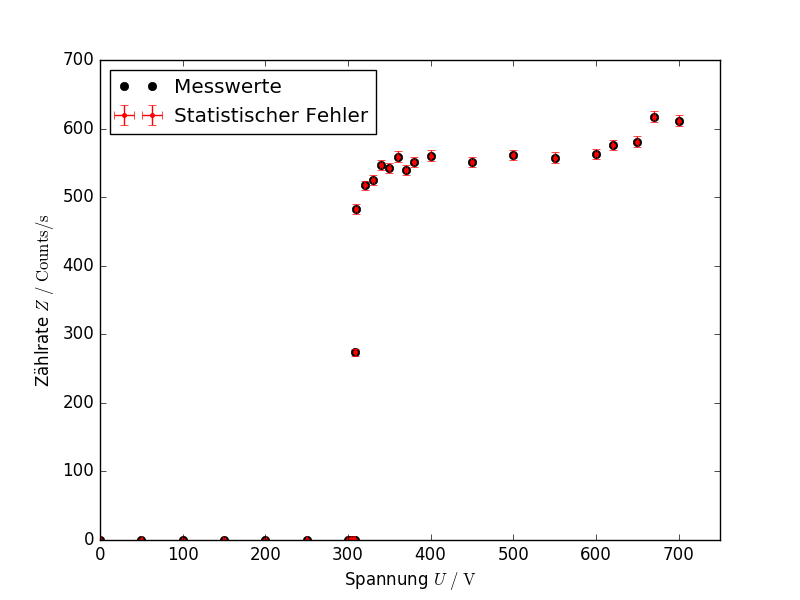
\includegraphics[width=0.8\textwidth]{build/charakteristik_gesamt.png}
	\caption{Alle Messdaten Zählrohr-Charakterisitk}
	\label{fig:charakteristik_gesamt}
\end{figure}



\begin{figure}[h!]
	\centering
	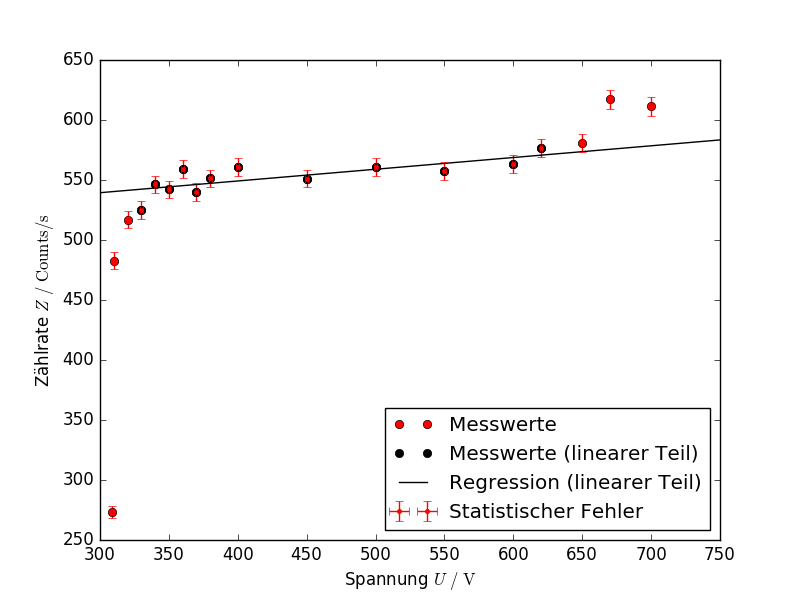
\includegraphics[width=0.8\textwidth]{build/charakteristik_linear.png}
	\caption{Regression an den linearen Anteil der Messdaten der Zählrohr-Charakterisitk. Die ausgenommenen Datenpunkte sind rot gekennzeichnet und die Daten, die in der Regression berücksichtigt sind, schwarz.}
	\label{fig:charakteristik_linear}
\end{figure}

\clearpage
Die Steigung des Plateaus wird mit Hilfe einer Regression an den linearen Teil der Messdaten (siehe Abbildung~\ref{fig:charakteristik_linear}) ermittelt. Die Regression und Fehlerrechnung wird mit Hilfe der Pythonversion 3.5.1 durchgeführt. Für die Regressionsvorschrift
\begin{align}
	Z = m \cdot U +b
\end{align}
folgen die Fit-Parameter
\begin{align}
	m &= \input{build/m1.txt}\quad , \\
	b &= \input{build/b1.txt} \quad .
\end{align}
Die Steigung $s$ soll nun in $\si{\percent}/\SI{100}{\volt}$ angegeben werden.
\begin{align}
	s = 100 \cdot \frac{Z_2 - Z_1}{Z_A} \cdot \frac{\si{\percent}}{\SI{100}{\volt}}
\end{align}
Hierbei entspricht $Z_A$ dem Wert der linearen Regression an der Stelle $U_A$, der Mitte des Plateaus, $Z_1$ dem Wert an der Stelle $U_A - \SI{50}{\volt}$ und $Z_2$ dem Wert zu $U_A + \SI{50}{\volt}$.

\begin{align}
	U_A = \input{build/U_mittel.txt} \quad Z_A = \input{build/Z_mittel.txt} \\
	U_1 = \input{build/U1.txt} \quad Z_1 = \input{build/Z1.txt} \\
	U_2 = \input{build/U2.txt} \quad Z2 = \input{build/Z2.txt}
\end{align}
Aus diesen Werten folgt eine Steigung von
\begin{align}
	s = \input{build/s.txt} \, \frac{\si{\percent}}{\SI{100}{\volt}} \quad .
\end{align}



\subsection{Zeit bis zur Nachentladung}
\todo{Ebberd möchte ausdrücklich nicht so kurze Sections -- eventuell direkt in die Diskussion.}
Die Zeit bis zur Nachentladung wird auf dem Oszilloskop abgelesen. Bei einer Spannung von \SI{350}{\volt} werden
\begin{align}
	t = \SI{70+-10}{\micro\second}
\end{align}
gemessen und bei einer Spannung von \SI{700}{\volt}
\begin{align}
	t = \SI{70+-10}{\micro\second} \quad .
\end{align}
Der Wert schwankte sehr stark und eventuell ist der Fehler sogar noch größer einzuordnen.

\clearpage 


\subsubsection{Bestimmung der Totzeit}
Die Totzeit $T$ wird auf zwei Arten bestimmt: Mit Hilfe einer Probe und dem Oszilloskop und mit Hilfe der Zählraten zweier Proben. \\
Das Ablesen am Oszilloskop liefert bei einer Spannung von \SI{700}{\volt} eine Totzeit von
\begin{align}
	T = \SI{30+-10}{\micro\second} \quad .
\end{align}
Für die Messung mit zwei Proben gilt
\begin{align}
	T = \frac{Z_1 + Z_2 - Z_{1+2}}{2 Z_1 Z_2}  \quad .
\end{align}
Bei einer Messzeit von 60 Sekunden wurden folgende Impulszahlen gemessen. Der Fehler entspricht wieder der Poisson-Statistik:
\begin{align*}
	N_1 = \num{14866+-122} \\
	N_{1+2} = \num{31548+-178} \\
	N_2 = \num{17281+-141}
\end{align*}
Mit $Z = N / \SI{60}{\second}$ folgt daraus eine Totzeit  von
\begin{align}
	T = \input{build/totzeit.txt} \quad .
\end{align}

\subsubsection{Freigesetzte Ladungen pro Impuls}
In einer letzten Messung wird zusätzlich zu der Anzahl der Impulsen $N$ der Strom $I$ gemessen, um herauszufinden, wie viele Elektronen mit der Elementarladung $e \approx  \SI{-1.602e-19}{\coulomb}$ durch ein Strahlungsteilchen freigesetzt werden. Die Messzeit beträgt 10 Sekunden. Mit $Q =  I \cdot t$ folgt:
\begin{align}
	\frac{\mathrm{Elekronen}}{\mathrm{Count}} = \frac{Q }{e \cdot \mathrm{Counts}} = \frac{I \cdot t }{e \cdot \mathrm{Counts}} \quad .
\end{align}
Die errechneten Werte sind in Tabelle~\ref{tab:ladungen} dargestellt. Der lineare Zusammenhang zwischen der angelegten Spannung und den registrieren Ladungen ist in Abbildung~\ref{fig:anzahl_elektronen} ersichtlich.



	 \begin{figure}[h!]
	 	\centering
	 	\captionof{table}{Messung zur Bestimmung der freigesetzten Ladungen pro Impuls}
	 	\begin{tabular}{cccc}
	 		$U \ /\  \mathrm{V}$ & N &  $I \ /\  \si{\micro\ampere}$ & $e \cdot 10^9$ \\
	 		\hline
	 		\input{build/tabelle_ladungen.txt}
	 	\end{tabular}
	 	\label{tab:ladungen}
	 \end{figure}
	 
	 \begin{figure}[h!]
	 	\centering
	 	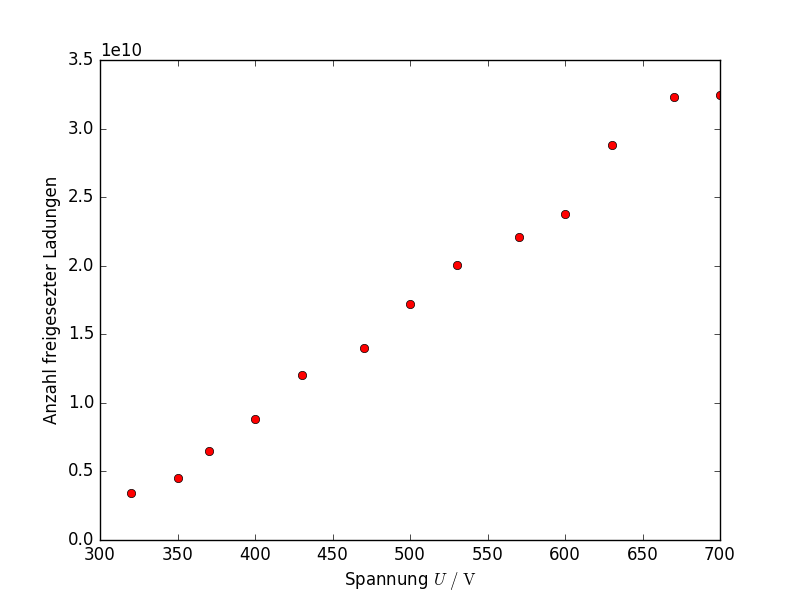
\includegraphics[width=0.8\textwidth]{build/anzahl_elektronen.png}
	 	\caption{Die Anzahl der registrierten Ladungen pro einfallendem Elektron der $\beta$-Strahlung in Abhängigkeit der angelegten Spannung}
	 	\label{fig:anzahl_elektronen}
	 \end{figure}




	
	